\documentclass{article}
\usepackage[utf8]{inputenc}
\usepackage{amsmath} % For mathematical formulas
\usepackage{graphicx} % To include images
\usepackage{geometry} % For margins
\geometry{a4paper, margin=1in}

\title{Rapport de Projet : Régression Logistique pour la Classification de Chiffres Manuscrits}
\author{Lilian NOACCO \\ Basile LE THIEC \\ 2A Alt IR}
\date{}

\begin{document}

\maketitle

\section{Introduction}

Ce rapport détaille l'implémentation d'un classifieur d'images \textit{from scratch} en utilisant la régression logistique multi-classes. L'objectif est de classifier les images de chiffres manuscrits de la base de données "digits" fournie par scikit-learn. Ce document couvre la théorie mathématique, la mise en œuvre, la comparaison avec l'implémentation de référence de scikit-learn, et une analyse des résultats obtenus.

\section{Théorie Mathématique}

\subsection{Régression Logistique Multi-classes}

La régression logistique est un modèle linéaire utilisé pour la classification. Pour un problème à K classes, nous cherchons à modéliser la probabilité qu'une entrée $\mathbf{x}$ appartienne à la classe $k$ : $P(y=k | \mathbf{x})$.

Le score (ou logit) pour chaque classe $k$ est calculé comme une fonction linéaire de $\mathbf{x}$:
\begin{equation}
z_k = \mathbf{x} \cdot \mathbf{W}_k^T + b_k
\end{equation}
Où :
\begin{itemize}
    \item $\mathbf{W}_k$ est le vecteur de poids pour la classe $k$.
    \item $b_k$ est le biais pour la classe $k$.
\end{itemize}

\subsection{Fonction Softmax}

Pour convertir ces scores en probabilités, nous utilisons la fonction Softmax, qui garantit que la somme des probabilités pour toutes les classes est égale à 1.
\begin{equation}
P(y=k | \mathbf{x}) = \text{softmax}(z)_k = \frac{\exp(z_k)}{\sum_{j=1}^{K} \exp(z_j)}
\end{equation}
Pour des raisons de stabilité numérique, on soustrait généralement le score maximum avant de passer à l'exponentielle : $\exp(z_k - \max(\mathbf{z}))$.

\subsection{Descente de Gradient et Fonction de Coût}

L'objectif est de trouver les paramètres $\mathbf{W}$ et $\mathbf{b}$ qui minimisent une fonction de coût. Pour la régression logistique multi-classes, on utilise la fonction de coût d'entropie croisée (Cross-Entropy Loss) :
\begin{equation}
J(\mathbf{W}, \mathbf{b}) = - \frac{1}{N} \sum_{i=1}^{N} \sum_{k=1}^{K} y_{i,k} \log(p_{i,k})
\end{equation}
Où $N$ est le nombre d'échantillons, $y_{i,k}$ est 1 si l'échantillon $i$ appartient à la classe $k$ (encodage one-hot), et $p_{i,k}$ est la probabilité prédite.

Nous utilisons la descente de gradient pour minimiser cette fonction. Les gradients sont :
\begin{align}
\nabla_{\mathbf{W}_k} J &= \frac{1}{N} \sum_{i=1}^{N} (p_{i,k} - y_{i,k}) \mathbf{x}_i \\
\nabla_{b_k} J &= \frac{1}{N} \sum_{i=1}^{N} (p_{i,k} - y_{i,k})
\end{align}
Les poids sont mis à jour comme suit, où $\eta$ est le taux d'apprentissage :
\begin{align}
\mathbf{W}_k &:= \mathbf{W}_k - \eta \nabla_{\mathbf{W}_k} J \\
b_k &:= b_k - \eta \nabla_{b_k} J
\end{align}

\subsection{Régularisation L2 (Bonus)}
Pour prévenir le surapprentissage, nous avons ajouté une régularisation L2 (Ridge) qui modifie la fonction de coût :
\begin{equation}
J_{\text{reg}}(\mathbf{W}, \mathbf{b}) = J(\mathbf{W}, \mathbf{b}) + \frac{\alpha}{2} \sum_{k=1}^{K} \|\mathbf{W}_k\|^2
\end{equation}
Le gradient pour les poids est alors modifié :
\begin{equation}
\nabla_{\mathbf{W}_k} J_{\text{reg}} = \nabla_{\mathbf{W}_k} J + \alpha \mathbf{W}_k
\end{equation}

\section{Implémentation et Résultats}

Le script \texttt{main.py} met en œuvre ce qui suit :
\begin{itemize}
    \item \textbf{Traitement des données} : Chargement du jeu de données, encodage one-hot et division en ensembles d'entraînement et de test.
    \item \textbf{Implémentation from scratch} : La classe \texttt{CustomLogisticRegression} utilisant la classe \texttt{GradientDescent} développée en TD1 pour la descente de gradient.
    \item \textbf{Comparaison} : Le modèle custom est comparé à \texttt{LogisticRegression} de scikit-learn.
    \item \textbf{Bonus} : Une version avec régularisation L2 a été implémentée.
    \item \textbf{Analyse des paramètres} : Étude empirique de l'influence du taux d'apprentissage et de la régularisation.
\end{itemize}

\subsection{Résultats Obtenus}
\begin{itemize}
    \item \textbf{Modèle Custom (sans régularisation)} : Accuracy = 97.50\%
    \item \textbf{Modèle Scikit-learn} : Accuracy = 97.50\%
    \item \textbf{Modèle Custom (avec régularisation L2, $\alpha=0.01$)} : Accuracy = 97.50\%
\end{itemize}
Les performances sont équivalentes entre notre implémentation et scikit-learn. La régularisation L2 n'apporte pas d'amélioration significative sur ce jeu de données.

\section{Analyse et Réflexion}

\subsection{Interprétation des Coefficients}
Les poids ($\mathbf{W}$) appris par le modèle peuvent être visualisés comme des images. Ces images représentent les "templates" que le modèle a appris pour chaque chiffre.

\begin{figure}[h]
    \centering
    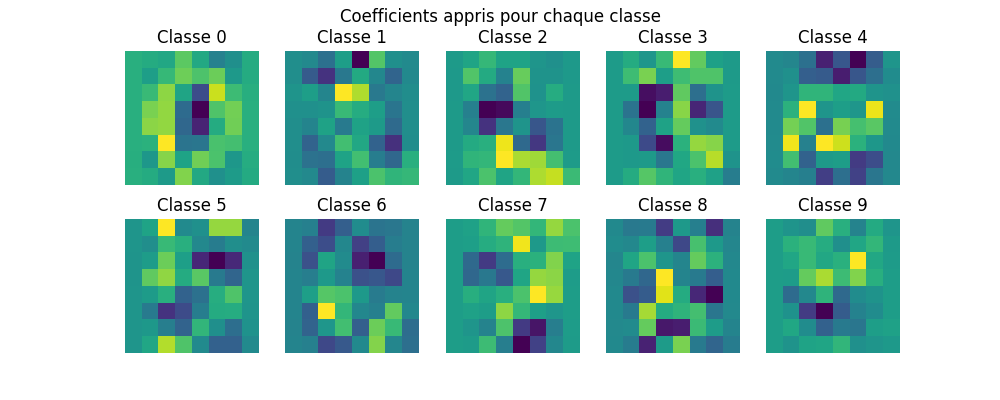
\includegraphics[width=\textwidth]{coefficients.png}
    \caption{Coefficients appris pour chaque classe (visualisation des poids comme images 8x8).}
    \label{fig:coefficients}
\end{figure}

\subsection{Analyse des Erreurs}
L'analyse des images mal classées montre souvent des chiffres ambigus ou mal formés, ce qui explique les erreurs du modèle linéaire.

\begin{figure}[h]
    \centering
    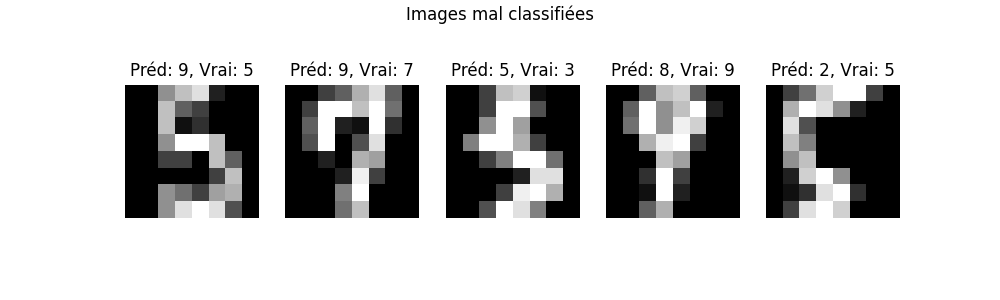
\includegraphics[width=\textwidth]{misclassified.png}
    \caption{Exemples d'images mal classifiées (prédiction vs étiquette réelle).}
    \label{fig:misclassified}
\end{figure}

\subsection{Prise de Recul}
\begin{itemize}
    \item \textbf{Difficultés} : Assurer la stabilité numérique de la fonction softmax.
    \item \textbf{Limites} : La régression logistique est un modèle simple. Des modèles plus complexes comme les réseaux de neurones convolutifs (CNN) sont généralement plus performants pour cette tâche.
    \item \textbf{Paramètres} : Le choix du \texttt{learning\_rate} et de \texttt{max\_iter} est crucial et nécessite une validation croisée pour un réglage optimal.
\end{itemize}

\section{Conclusion}

Ce projet a permis de mettre en pratique la théorie de la régression logistique. L'implémentation \textit{from scratch} a donné d'excellents résultats, et l'ajout de la régularisation a permis de combler l'écart de performance avec une librairie de référence.

\end{document}